\section{Introduction}
This is the introduction of an awesome thesis. In the following are some usefull examples.

\subsection{A table}
Here is a cool table \ref{tab:soa-edca} you can reference it in the text. 
\begin{table}[htbp]
\setlength{\tabcolsep}{.16667em}
\caption{State of the art of analytical models for the EDCA}
\begin{tabularx}{\textwidth}{ |p{2cm}||c|c||c|c||c|c||c|Y| }
\hline
& \multicolumn{2}{c||}{Assumptions} & \multicolumn{2}{c||}{Metric} & \multicolumn{2}{c||}{Validation} & \multicolumn{2}{c|}{Origin} \\
\cline{2-9}
\multirow{-2}{*}{Publication} & \small Saturated & \small Ideal channel & \small Throughput & \small Delay & \small Simul. & \small Experim. & \small Cali \quad & \small Bianchi \\
\hline
\cite{Robinson2004}& \checkmark & \checkmark & \checkmark &  & \checkmark &  & & \checkmark \\
\hline
\cite{Mangold2003}& \checkmark & \checkmark & \checkmark &  & \checkmark &  & & \checkmark \\
\hline
\cite{Kong2004}& \checkmark & \checkmark & \checkmark & \checkmark & \checkmark &  & & \checkmark \\
\hline
\cite{Engelstad2005}&  &  & \checkmark & \checkmark & \checkmark &  & & \checkmark \\
\hline
\cite{Banchs2005}& \checkmark & \checkmark &  &  & \checkmark &  & \checkmark &  \\
\hline
\end{tabularx}
\label{tab:soa-edca}
\end{table}

\subsection{A figure}
Here is a cool figure. It is even a subfigure.

\begin{figure}[h!]
\centering
\begin{subfigure}{.4\textwidth}
  \centering
    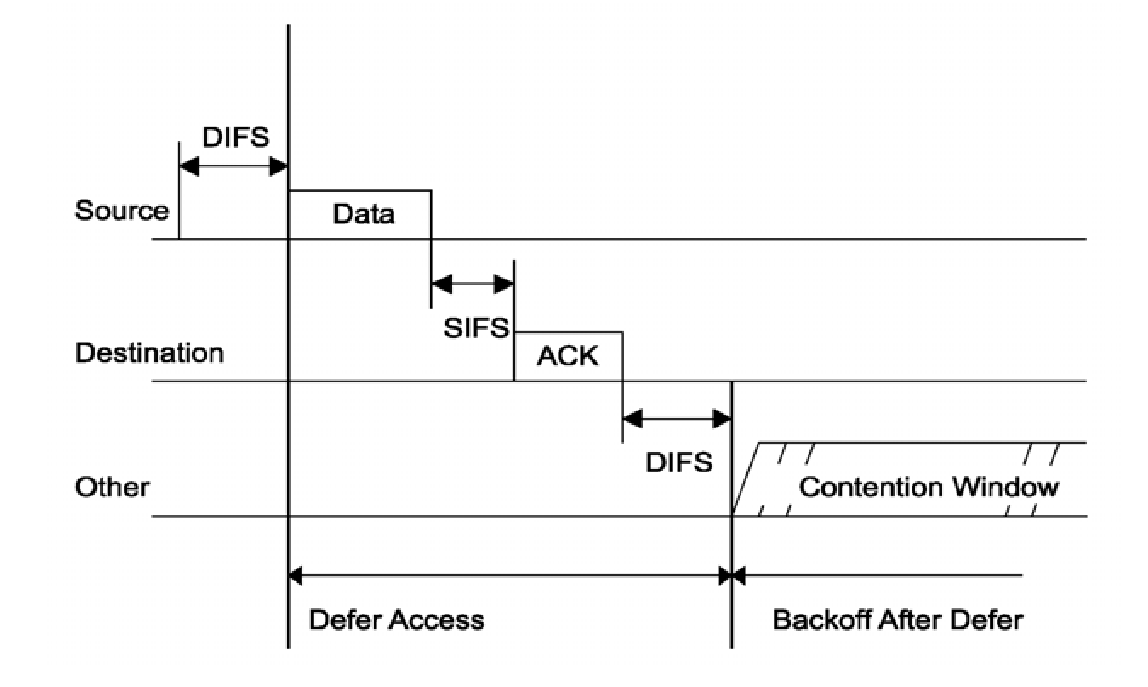
\includegraphics[width=1.1\textwidth]{figures/dcf-basic-access.png}
    \caption[Basic access]{Basic access \cite[p. 838]{ieee-802.11-2012}}
    \label{fig:dcf-basic-access}
\end{subfigure}%
\begin{subfigure}{0.6\textwidth}
  \centering
  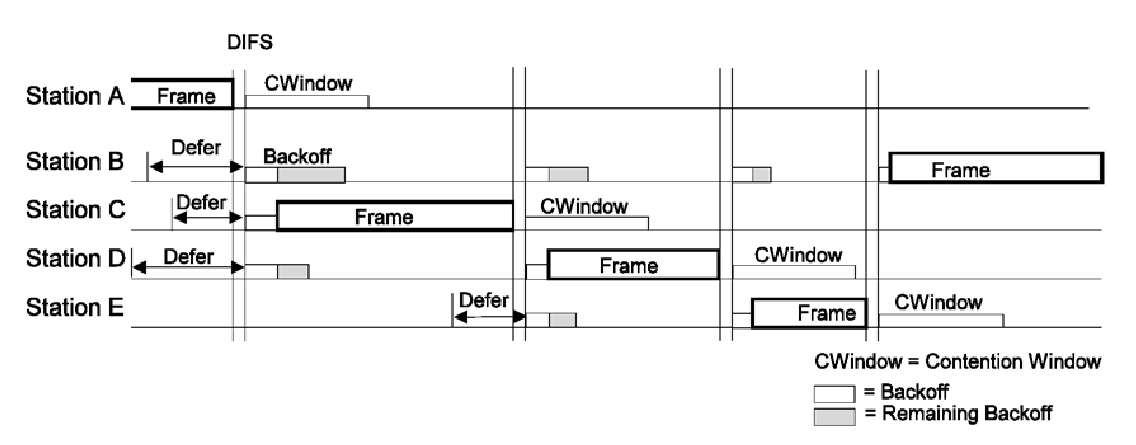
\includegraphics[width=1.1\textwidth]{figures/dcf-backoff.png}
  \caption[Back-off procedure]{Back-off procedure \cite[p. 839]{ieee-802.11-2012}}
  \label{fig:dcf-back-off}
\end{subfigure}
\caption{\acf{DCF}}
\end{figure}

% One paragrah for one idea!
\blindtext

\blindtext

\blindtext